%%%%%%%%%%%%%%%%%%%%%%%%%%%%%%%%%%%%%%%%%%%%%%%%%%%%%%%%%%%%%%%%%%%%%%
% LaTeX Example: Class Summary
%
% Source: http://www.howtotex.com
%
% Feel free to distribute this example, but please keep the referral
% to howtotex.com
% Date: February 2018
% 
%%%%%%%%%%%%%%%%%%%%%%%%%%%%%%%%%%%%%%%%%%%%%%%%%%%%%%%%%%%%%%%%%%%%%%
% How to use writeLaTeX: 
%
% You edit the source code here on the left, and the preview on the
% right shows you the result within a few seconds.
%
% Bookmark this page and share the URL with your co-authors. They can
% edit at the same time!
%
% You can upload figures, bibliographies, custom classes and
% styles using the files menu.
%
% If you're new to LaTeX, the wikibook is a great place to start:
% http://en.wikibooks.org/wiki/LaTeX
%
%%%%%%%%%%%%%%%%%%%%%%%%%%%%%%%%%%%%%%%%%%%%%%%%%%%%%%%%%%%%%%%%%%%%%%
% Edit the title below to update the display in My Documents
%\title{Project Report}
%
%%% Preamble
\documentclass[paper=a4, fontsize=11pt]{scrartcl}
\usepackage[T1]{fontenc}
\usepackage{fourier}

\usepackage[english]{babel}															% English language/hyphenation
\usepackage[protrusion=true,expansion=true]{microtype}	
\usepackage{amsmath,amsfonts,amsthm} % Math packages
\usepackage{amssymb,mathtools}
\usepackage[pdftex]{graphicx}	
\usepackage{url}
\usepackage{listings}
\usepackage{float}
\usepackage{enumitem}
\usepackage[usenames, dvipsnames]{color}
%%% Custom sectioning
\usepackage{sectsty}
\allsectionsfont{\centering \normalfont\scshape}


%%% Custom headers/footers (fancyhdr package)
\usepackage{fancyhdr}
\pagestyle{fancyplain}
\fancyhead{}											% No page header
\fancyfoot[L]{}											% Empty 
\fancyfoot[C]{}											% Empty
\fancyfoot[R]{\thepage}									% Pagenumbering
\renewcommand{\headrulewidth}{0pt}			% Remove header underlines
\renewcommand{\footrulewidth}{0pt}				% Remove footer underlines
\setlength{\headheight}{13.6pt}


%%% Equation and float numbering
\numberwithin{equation}{section}		% Equationnumbering: section.eq#
\numberwithin{figure}{section}			% Figurenumbering: section.fig#
\numberwithin{table}{section}				% Tablenumbering: section.tab#

%%% Images
\usepackage{graphicx}
\graphicspath{ {/home/kushal/Unconstrained_Optimization_ECE505/Report} }

%%% Maketitle metadata
\newcommand{\horrule}[1]{\rule{\linewidth}{#1}} 	% Horizontal rule

\title{
		%\vspace{-1in} 	
		\usefont{OT1}{bch}{b}{n}
		\normalfont \normalsize \textsc{IIT/ECE505 Computer Project - I} \\ [25pt]
		\horrule{0.5pt} \\[0.4cm]
		\huge Unconstrained Optimization Algorithms \\
		\horrule{2pt} \\[0.5cm]
}


\author{
        \\[150pt]
        \normalfont 								\normalsize
        Kushal Virupakshappa\\[-3pt]		        \normalsize
        CWID: A20305737\\[-3pt]		                \normalsize
        Instructor/Professor: Yongyi Yang\\[-3pt]		    \normalsize
        T.A: Amin Zarshenas\\[-3pt]		            \normalsize        
}
\date{November 5, 2018}

%%% Begin document
\begin{document}
\maketitle
\section*{Acknowledgement}

I here by acknowledge that neither any assistance has been taken from other people nor has been copied from any other source available on the internet. The sentences written in this report are my own and the work/paper/journal referred to are cited in the bibliography.\\[5pt]





Kushal Virupakshappa

\today
\date{}



\clearpage
\vspace*{2.5cm}

\section*{Abstract}
This work focuses on the implementation of the Unconstrained Optimization alogrithms. Steepest Gradient Descent Optimization, Newton's Optimiztion, BFGS Optimization and Conjugate Gradient Method Optimization methods are the specific algorithms which have been used in this work. Newton's line search method with Armijo Condition has been used to decide descent step in a given direction with the Steepest Gradient Descent and BFGS methods. For most the problem cases the convergence criteria has been met and for few problems the maximum iteration limit was reached. The convergence rate depends on the kind of optimization function and optimization algorithm. \\
\section{Keywords}
Steepest Gradient Descent (SGD) Optimization, Newton's Optimization,BFGS Optimization, Conjugate Gradient Method (CGD) Optimization, Maximum Likelihood Estimation (MLE), Log Likelihood and Expectation-Maximization (EM) algorithm.
\section{Software Tools and Libraries}
The software Tools and the libraries used in this project are listed below:
\paragraph{Software Tools\newline}
Python, Anaconda Environment, Jupyter Notebook.
\paragraph{Libraries\newline}
Numpy, Matplotlib.\newline
More details regarding setup are given in readme.md file in \cite{last}.
\section{Problem statement}
There are two parts for the project. Part 1 involves implementing SGD, Newton, BFGS and CGD algorithms as described in \cite{one}. Part 2 involves application of the optimization algorithm to identify regions of cancerous and non cancerous pixels by estimating mean and variance for each region. The Optimization problems for each part are listed below.
\subsection{Part 1 Optimization Problems}
The following equations are used in optimization as given in the project problems.
\begin{align}
\label{eqn:e1}
\begin{split}
 f_{(1)}(\vec{x})=x_1^2+x_2^2+x_3^2 ,
\\
 \vec{x_0}=(x_1,x_2,x_3)_0^T=(1,1,1)^T.
\end{split}
\end{align}
\begin{align}
\label{eqn:e2}
\begin{split}
 f_{(2)}(\vec{x})=x_1^2 + 2*x_2^2 - 2*x_1*x_2 - 2*x_2,
\\
 \vec{x_0}=(x_1,x_2)_0^T=(0,0)^T.
\end{split}
\end{align}
\begin{align}
\label{eqn:e3}
\begin{split}
 f_{(3)}(\vec{x})=100*(x_2-x_1^2)^2 + (1-x_1)^2 ,
\\
 \vec{x_0}=(x_1,x_2)_0^T=(-1.2,1)^T.
\end{split}
\end{align}
\begin{align}
\label{eqn:e4}
\begin{split}
 f_{(4)}(\vec{x})=(x_1 + x_2)^4 + x_2^2 ,
\\
 \vec{x_0}=(x_1,x_2)_0^T=(2,-2)^T.
\end{split}
\end{align}
\begin{align}
\label{eqn:e5}
\begin{split}
 f_{(5)}(\vec{x})=(x_1 - 1)^2 + (x_2 - 1)^2 + c*(x_1^2+x_2^2-0.25)^2 ,
\\
 \vec{x_0}=(x_1,x_2)_0^T=(1,-1)^T,c=1,10,100.
\end{split}
\end{align}

\subsection{Part 2 Optimization Problem}
The problem statement involves finding estimates of $\mu_1$, $\sigma_1^2$,$\mu_2$, $\sigma_2^2$ and $P$ in the Probability Distribution Function(PDF) given in Eq.\ref{eqn:e6}. In Eq.\ref{eqn:e6} $i$ refers to the samples of the pixels in the mamography image provided in xls file.
\begin{align}
\label{eqn:e6}
\begin{split}
 p(x_i;\mu_1,\sigma_1^2,\mu_2,\sigma_2^2,P)= P \frac{1}{\sqrt{2\pi\sigma_1^2}} e^{\frac{-(x_i-\mu_1)^2}{2 \sigma_1^2}}+(1-P) \frac{1}{\sqrt{2\pi\sigma_2^2}} e^{\frac{-(x_i-\mu_2)^2}{2 \sigma_2^2}}
\\
 \Theta=(\mu_1,\sigma_1^2,\mu_2,\sigma_2^2,P)=\underset{\Theta}{argmax} (\Pi_{i=1}^{200} p(x_i;\mu_1,\sigma_1^2,\mu_2,\sigma_2^2,P))
\end{split}
\end{align}

According to \cite{two}, since the log likelihood Eq.\ref{eqn:e6} does not converge a new random variable $Z$ is introduced such that $Z={0,1}$ and by using joint distribution and posterior probability a new algorithm called EM algorithm is introduced which reduces the optimization to maximizing $Q$ or minimizing $-Q$ of Eq.\ref{eqn:e7}. The Expectation step of EM algorithm includes calculation Eq.\ref{eqn:e8} using the parameters calculated in Maximization/Minimization step.
 
\begin{align}
\label{eqn:e7}
Q(\Theta,\Theta_{old})=\Sigma_{i=1}^{200}\Sigma_{k=1}^{2}((ln(P_k)+\frac{1}{2}ln(2\pi\sigma_k^2)-\frac{(x_i-\mu_k)^2}{2\sigma_k^2})(p_{ik}(z/x_i;\Theta_{old}))
\end{align}

\begin{align}
\label{eqn:e8}
p_{ik}(z/x_i;\Theta_{old})=\frac{P_k*GaussPDF(x_{ik};\Theta_{old})}{\Sigma_{i=1}^{200}\Sigma_{k=1}^{2}P_k*GaussPDF(x_{ik;\Theta_{old}})}
\end{align}

\section{Algorithms}
Each of the algorithms used in this work are described in this section. SGD, Newton, BFGS, CGD, Newton's Line Search and Armijo condition algorithms are derived and detailed in \cite{one}. EM algorithm used in application problem is described in \cite{two}.

\paragraph{Steepest Gradient Descent Optimization method}
\begin{enumerate}
  \item Initialize the parameters to be optimized and $\alpha$ which is the line search step.
  \item Check if $\frac{||{\triangledown f(\vec{x})}||}{1+|f(x)|}$ or Maximum Iteration reached.If yes the parameters are optimized else go to next step.
  \item Compute direction vector $\vec{p}$ by using gradient of the optimization function using gradient of the function as given in $\vec{p}=-\bigtriangledown f(\vec{x})$.
  \item Compute $\alpha$ using Newton's Line search method with Armijo Condition.
  \item Compute $\vec{x_{new}}=\vec{x_{old}}+\alpha\vec{p}$.
  \item Repeat step2.
\end{enumerate}

\paragraph{Newton's Optimization method}

\begin{enumerate}
  \item Initialize the parameters to be optimized.
  \item Check if $\frac{||{\triangledown f(\vec{x})}||}{1+|f(x)|}$ or Maximum Iteration reached.If yes the parameters are optimized else go to next step.
  \item Compute $\bigtriangledown f(\vec{x})$ for current value of parameters.
  \item Compute $\bigtriangledown^2 f(\vec{x})$,which is the hessian matrix of the given function for current value of parameters.
  \item Compute $\vec{x_{new}}=\vec{x_{old}}-[\bigtriangledown^2 f(\vec{x})]^{-1} \bigtriangledown f(\vec{x})$.
  \item Repeat step2.
\end{enumerate}

\paragraph{BFGS Quasi-Newton Optimization method}
\begin{enumerate}
  \item Initialize the parameters to be optimized, matrix $B$ and $\alpha$ which is the line search step.
  \item Check if $\frac{||{\triangledown f(\vec{x})}||}{1+|f(x)|}$ or Maximum Iteration reached.If yes the parameters are optimized else go to next step.
  \item Compute direction vector $\vec{p}$ by solving the equation $B\vec{p}=-\triangledown f(\vec{x})$.
  \item Compute $\alpha$ using Newton's Line search method with Armijo Condition.
  \item Compute $\vec{x_{new}}=\vec{x_{old}}+\alpha\vec{p}$.
  \item Compute $B_{new}=B_{old}-\frac{(B_{old}s)(B_{old}s)^T}{(s^TB_{old}s)}+\frac{yy^T}{y^Ts}$, where $s=\vec{x_{new}}-\vec{x_{old}}$ and $y=\triangledown f(\vec{x_{new}})-\triangledown f(\vec{x_{old}})$.
  \item Repeat step2.
\end{enumerate}

\paragraph{Conjugate Gradient Descent Optimization method}
\begin{enumerate}
  \item Initialize the parameters to be optimized and direction vector to negetive ofgradient of initialized parameters i.e.,$d_0=-\triangledown f(\vec{x})$.
  \item Check if $\frac{||{\triangledown f(\vec{x})}||}{1+|f(x)|}$ or Maximum Iteration reached.If yes the parameters are optimized else go to next step.
  \item Compute $\bigtriangledown^2 f(\vec{x})$,which is the hessian matrix of the given function for current value of parameters.
  \item Compute $\alpha$ using $\alpha=\frac{-d_i \triangledown f(\vec{x})}{d_i^T\bigtriangledown^2 f(\vec{x})d_i}$.
  \item Compute $\vec{x_{new}}=\vec{x_{old}}+\alpha\vec{p}$.
  \item Compute $\beta$ using $\beta=\frac{d_i \triangledown f(\vec{x_{new}})}{d_i^T\bigtriangledown^2 f(\vec{x_{new}})d_i}$.
  \item Compute $d_{i+1}=-\triangledown f(\vec{x_{new}})+ \beta d_i$
  \item Repeat step2.
\end{enumerate}

\paragraph{Newton's Line Search method}
\begin{enumerate}
  \item Initialize the parameters to be optimized.
  \item Check if Armijo Condition is met if yes terminate with latest alpha else continue.
  \item Compute $\bigtriangledown f(\alpha)$ for current value of parameters.
  \item Compute $\bigtriangledown^2 f(\alpha)$,which is the hessian matrix of the given function for current value of parameters.
  \item Compute $\alpha_{new}=\alpha_{old}-[\bigtriangledown^2 f(\alpha_{old})]^{-1} \bigtriangledown f(\alpha_{old})$.
  \item Repeat step2.
\end{enumerate}

\paragraph{Armijo Condition}
\begin{enumerate}
  \item $f(\vec{x}+\alpha \vec{p})<=f(\vec{x})+\mu \alpha \vec{p}^T \bigtriangledown f(\vec{x})$
  \item If above condition is satisfied return True else return False.
\end{enumerate}
\paragraph{Expectation Maximization Method}
\begin{enumerate}
  \item Choose an initial parameters $\Theta$.
  \item E step(Expectation step): Compute $p_{ik}(z/x_i;\Theta_{old})$ using Eq.\ref{eqn:e8}.
  \item M step(Maximization or Minimization step): Minimize function $-Q(\Theta;\Theta_{old})$ given in Eq.\ref{eqn:e7} w.r.t $\Theta$.
  \item Check for convergence if yes exit else repeat from step 2.
\end{enumerate}
\section{Results}

The results for each optimization problem with respect of each algorithm has been provided in this section.\textbf{The screen shot of the ouput is attached in the Appendix section. Only sample examples are attached for Eq.\ref{eqn:e1} in this section.}

\paragraph{Results for Optimization problem in Eq.\ref{eqn:e1}\newline}
\textbf{The convergence is achieved in 1 iteration for SGD,BFGS and CGD while Newton's method achievied convergence at 19th iteration}. The outputs can be seen in Figure.\ref{out1} and Figure .\ref{out2} for Eq.\ref{eqn:e1}.The convergence value of $\vec{x}$ is $\vec{x}=[0,0,0]^T$
\begin{figure}[H]
\caption{Output of SGD, Newton, BFGS and CGD optimization}
\centering
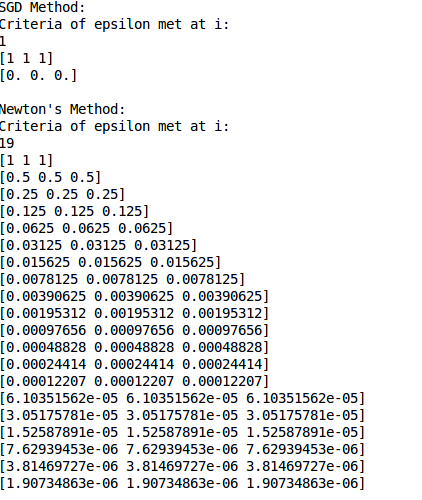
\includegraphics[width=0.25\textwidth]{out1.png}
\label{out1}
\end{figure}
\begin{figure}[H]
\caption{Output of SGD and Newton optimization}
\centering
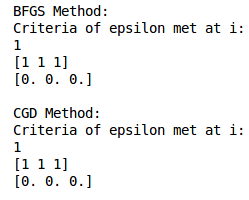
\includegraphics[width=0.25\textwidth]{out2.png}
\label{out2}
\end{figure}
\paragraph{Results for Optimization problem in Eq.\ref{eqn:e2}\newline}
\textbf{The convergence is achieved in 52,54,39 and 33 iterations respectively for SGD,Newton,BFGS and CGD}. The outputs can be seen in Figure.\ref{out3} and Figure .\ref{out4} for Eq.\ref{eqn:e2}.The convergence value of $\vec{x}$ is $\vec{x}=[1,1]^T$
\paragraph{Results for Optimization problem in Eq.\ref{eqn:e3}\newline}
\textbf{The convergence is not achieved for SGD,Newton and BFGS but for CGD convergence is achieved at 430th iteration}. The outputs can be seen in Figure.\ref{out5} and Figure .\ref{out6} for Eq.\ref{eqn:e3}.The convergence value of $\vec{x}$ is $\vec{x}=[1,1]^T$
\paragraph{Results for Optimization problem in Eq.\ref{eqn:e4}\newline}
\textbf{The convergence is not achieved for SGD,Newton but for BFGS and CGD convergence is achieved at 42nd and379th iteration}. The outputs can be seen in Figure.\ref{out7},Figure.\ref{out8},Figure.\ref{out9} and Figure .\ref{out10} for Eq.\ref{eqn:e4}.The convergence value of $\vec{x}$ is $\vec{x}=[1.5*10^{-2},0]^T$
\paragraph{Results for Optimization problem in Eq.\ref{eqn:e5}\newline}
\begin{enumerate}
  \item \textbf{For c=1, the output converges for SGD,Newton,BFGS and CGD at 19,124,65 and 15 iteration respectively.}The convergence value of $\vec{x}$ is $\vec{x}=[0.564,0.564]^T$.The outputs can be seen in Figure.\ref{out11} and Figure .\ref{out12}
  \item \textbf{For c=10, the output converges for SGD,Newton,BFGS and CGD at 85,715,563 and 14 iteration respectively.}The convergence value of $\vec{x}$ is $\vec{x}=[0.4026,0.4026]^T$.The outputs can be seen in Figure.\ref{out13} and Figure .\ref{out14}
  \item \textbf{For c=100, the output of Newton and BFGS doesn't converge while output of SGD and CGD converges at 863 and 223 iterations respectively.}The convergence value of $\vec{x}$ is $\vec{x}=[0.3597,0.3597]^T$.The outputs can be seen in Figure.\ref{out14} and Figure .\ref{out15}
\end{enumerate}
\paragraph{Results for Application(optional) Problem\newline}
The Application problem is delt using EM algorithm with Q function optimized using Steepest Gradient Descent Method for Maximization step.The algorithm was started with seed value of $\Theta=(\mu_1,\sigma_1^2,\mu_2,\sigma_2^2,P)=(100,50,150,50,0.5)$. After 1000 iterations of EM algorithm there was no convergence but the new $\Theta$ value is  $\Theta=(120.261310,196.28040,201.659041,218.19920,0.6165765)$.The output can be seen in Figure.\ref{out18}
\section{Evaluation of Results}
\begin{itemize}
  \item It can be observed that SGD decreases at linear rate for all the optimization problems.Hence slower compared to all other methods in cases where the condition of Q or Hessian matrix is comparetively smaller as in Eq.\ref{eqn:e1},Eq.\ref{eqn:e2} and Eq.\ref{eqn:e3}. It is still linear in Higher values for condition of Q but BFGS and Newton's method might fail to converge.
  \item Newton's method in theory should converge at quadratic rate but even for simple case as in Eq.\ref{eqn:e1} it is severely limited by the precision or accuracy while in other cases there are intermediary hessian matrix which may not be singular thus triggering unwanted outputs and hence will not converge as in Eq.\ref{eqn:e3}
  \item BFGS method does well for most of the cases but fails to converge whenever the matrix B is not singular as in Eq.\ref{eqn:e3}. Compared to SGD it does well in most of the cases but the convergence rate slows done for the cases where condition of Q is high.
  \item CGD converges in all the cases and outperforms all the methods taking fewer number of steps when compared to other algorithms and matches theoretical explanation that it converges in fixed number of steps.
  \item Though the EM alogrithm didnot converge it has given new $\Theta$ value which is pretty close to the visual histogram representation of data as shown in Figure.\ref{out17}.  
\end{itemize}
\begin{figure}[H]
\caption{Histogram of Mammogram pixel samples}
\centering
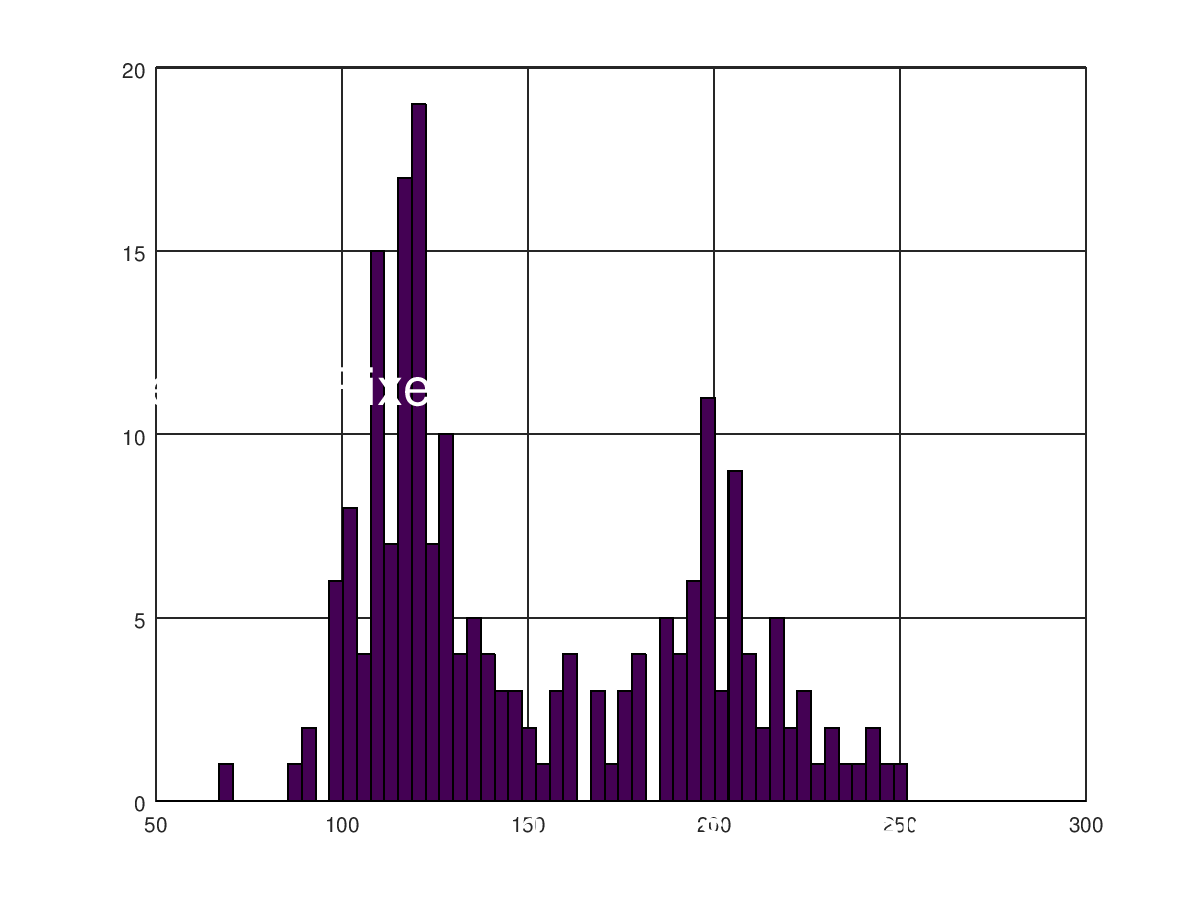
\includegraphics[width=0.75\textwidth]{histogram.png}
\label{out17}
\end{figure}

\section{Conclusion}
The algorithms implemented work as expected to theory but the rate of convergence is effected by accuarcy for Newton's method which downplays the strength of Newton's optimization implementation in practical scenarios.The rest of the algorithms hold up their end of the promises matching the theory for all the scenarios and having pitfalls as explained in theory and the Newton's Line Search method with Armijo condition works according to the theory and is limited by the seed values of $\alpha$ and $\mu$ as there are situtions where the Armijo condition may not get satisfied,This was resolved by keeping the $\mu$ as low as possible for given optimization problem or by changing the seed value of optimizing parameters.The EM algorithm works as expected and moves toward acheiving the Maximum Likelihood Estimate and is limited only by the kind of optimization algorithm used to solve the maximization of Q function. \\

\section{Future Work}
\begin{enumerate}
   \item Implement Secant method of Line search and Wolfe Condition to check the validity of the implemented algorithms for given optimization problems.
   \item Implement EM algorithm with CGD method to optimize Q function so that convergence can be achieved.
   \item Calculate the convergence rate for each algorithm using the formulas provided in the \cite{one} and verify the convergence rate for each function and algorithm.
\end{enumerate}

\begin{thebibliography}{100}  % 100 is a random guess of the total number of 
%references
\bibitem{one} Griva.I, Nash .S.G,and Sofer .A,"Linear and Non Linear Optimization," \emph{Society for Industrial and Applied Mathematics},2nd Ed,ISBN 978-0-898716-61-0,2009.
\bibitem{two} Bishop,C.,"Pattern Recognition and Machine Learning," \emph{Springer},ISBN-10: 0-387-31073-8,Pg. 430-443,February 2006.
\bibitem{last} Virupakshappa .K,"Github link to Project Source Code and Useage," \url{https://github.com/kushalviit/Unconstrained_Optimization_ECE505.git}.
\end{thebibliography}

\section*{Appendix}
The source code can be downloaded and used/tested by using the GitHub link in \cite{last}.
Since the number of code lines is large link has been provided to Github jupyter notebook or see the python file source\_code.py attached separately.
\subsection*{Source Code of all the four optimization algorithms}
\textbf{\url{https://github.com/kushalviit/Unconstrained_Optimization_ECE505/blob/master/project_notebook.ipynb}
Go to PART1-Algorithmic Implementation 1.All the Optimization Algorithm}
\subsection*{Source Code of all the four optimization algorithms}
\textbf{\url{https://github.com/kushalviit/Unconstrained_Optimization_ECE505/blob/master/project_notebook.ipynb}
Go to 2.Function 1 by scrolling down}
\subsection*{Images of outputs for Optimization problem in Eq.\ref{eqn:e2} and Source Code}
\textbf{Source Code: \url{https://github.com/kushalviit/Unconstrained_Optimization_ECE505/blob/master/project_notebook.ipynb}
Go to 3.Function 2 by scrolling down}

\begin{figure}[H]
\caption{Output of SGD and Newton optimization}
\centering
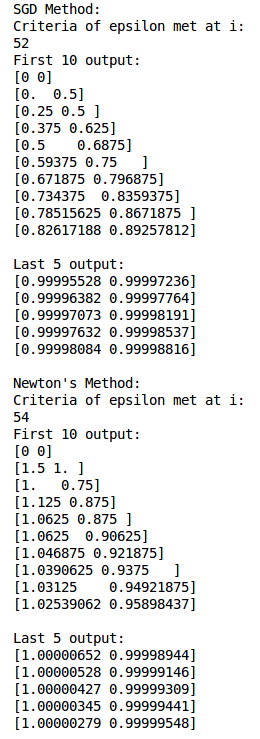
\includegraphics[width=0.25\textwidth]{out3.png}
\label{out3}
\end{figure}
\begin{figure}[H]
\caption{Output of BFGS and CGD optimization}
\centering
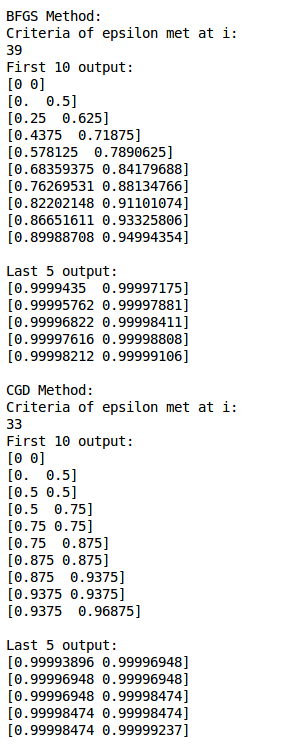
\includegraphics[width=0.25\textwidth]{out4.png}
\label{out4}
\end{figure}
\subsection*{Images of outputs for Optimization problem in Eq.\ref{eqn:e3} and Source Code}
\textbf{Source Code: \url{https://github.com/kushalviit/Unconstrained_Optimization_ECE505/blob/master/project_notebook.ipynb}
Go to 4.Function 3 by scrolling down}

\begin{figure}[H]
\caption{Output of SGD and Newton optimization}
\centering
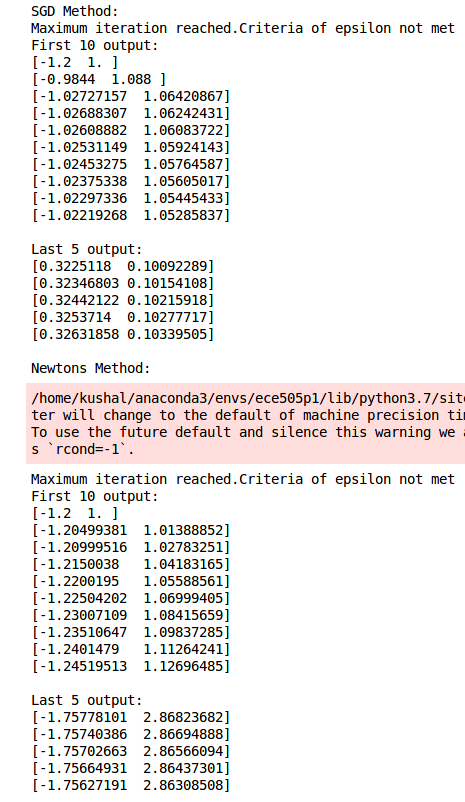
\includegraphics[width=0.25\textwidth]{out5.png}
\label{out5}
\end{figure}
\begin{figure}[H]
\caption{Output of BFGS and CGD optimization}
\centering
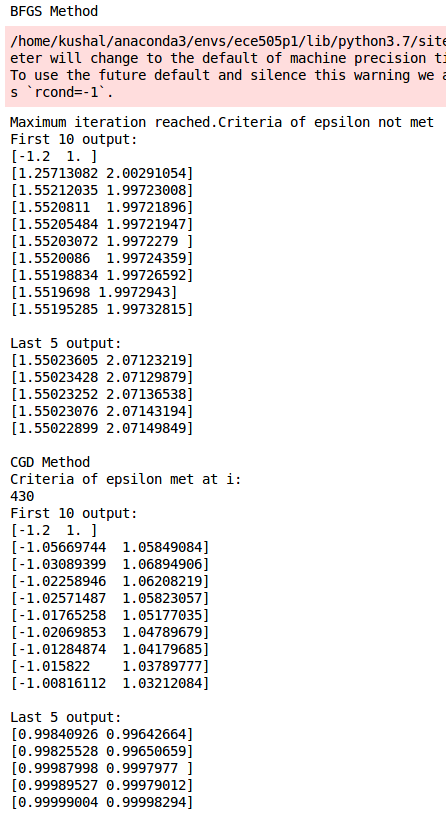
\includegraphics[width=0.25\textwidth]{out6.png}
\label{out6}
\end{figure}
\subsection*{Images of outputs for Optimization problem in Eq.\ref{eqn:e4} and Source Code}
\textbf{Source Code: \url{https://github.com/kushalviit/Unconstrained_Optimization_ECE505/blob/master/project_notebook.ipynb}
Go to 5.Function 4 by scrolling down}

\begin{figure}[H]
\caption{Output of SGD optimization}
\centering
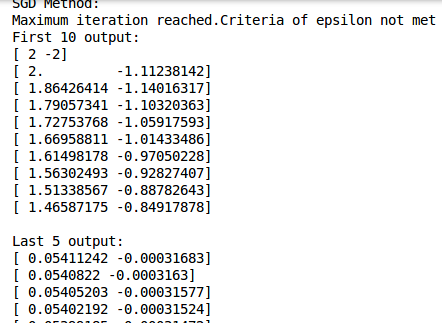
\includegraphics[width=0.25\textwidth]{out7.png}
\label{out7}
\end{figure}
\begin{figure}[H]
\caption{Output of Newton optimization}
\centering
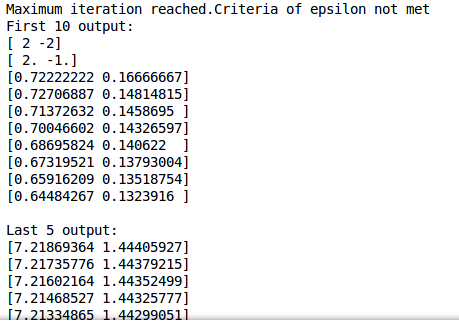
\includegraphics[width=0.25\textwidth]{out8.png}
\label{out8}
\end{figure}
\begin{figure}[H]
\caption{Output of BFGS optimization}
\centering
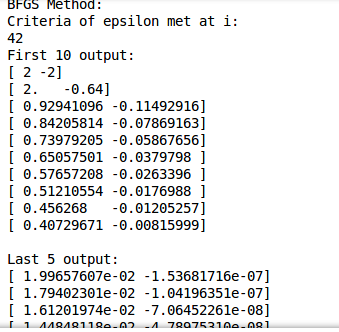
\includegraphics[width=0.25\textwidth]{out9.png}
\label{out9}
\end{figure}
\begin{figure}[H]
\caption{Output of CGD optimization}
\centering
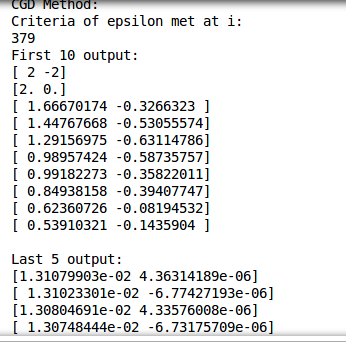
\includegraphics[width=0.25\textwidth]{out10.png}
\label{out10}
\end{figure}

\subsection*{Images of outputs for Optimization problem in Eq.\ref{eqn:e5} and Source Code}
\textbf{\url{https://github.com/kushalviit/Unconstrained_Optimization_ECE505/blob/master/project_notebook.ipynb}
Go to 6.Function 5 by scrolling down}
\begin{figure}[H]
\caption{Output of SGD and Newton optimization for C=1}
\centering
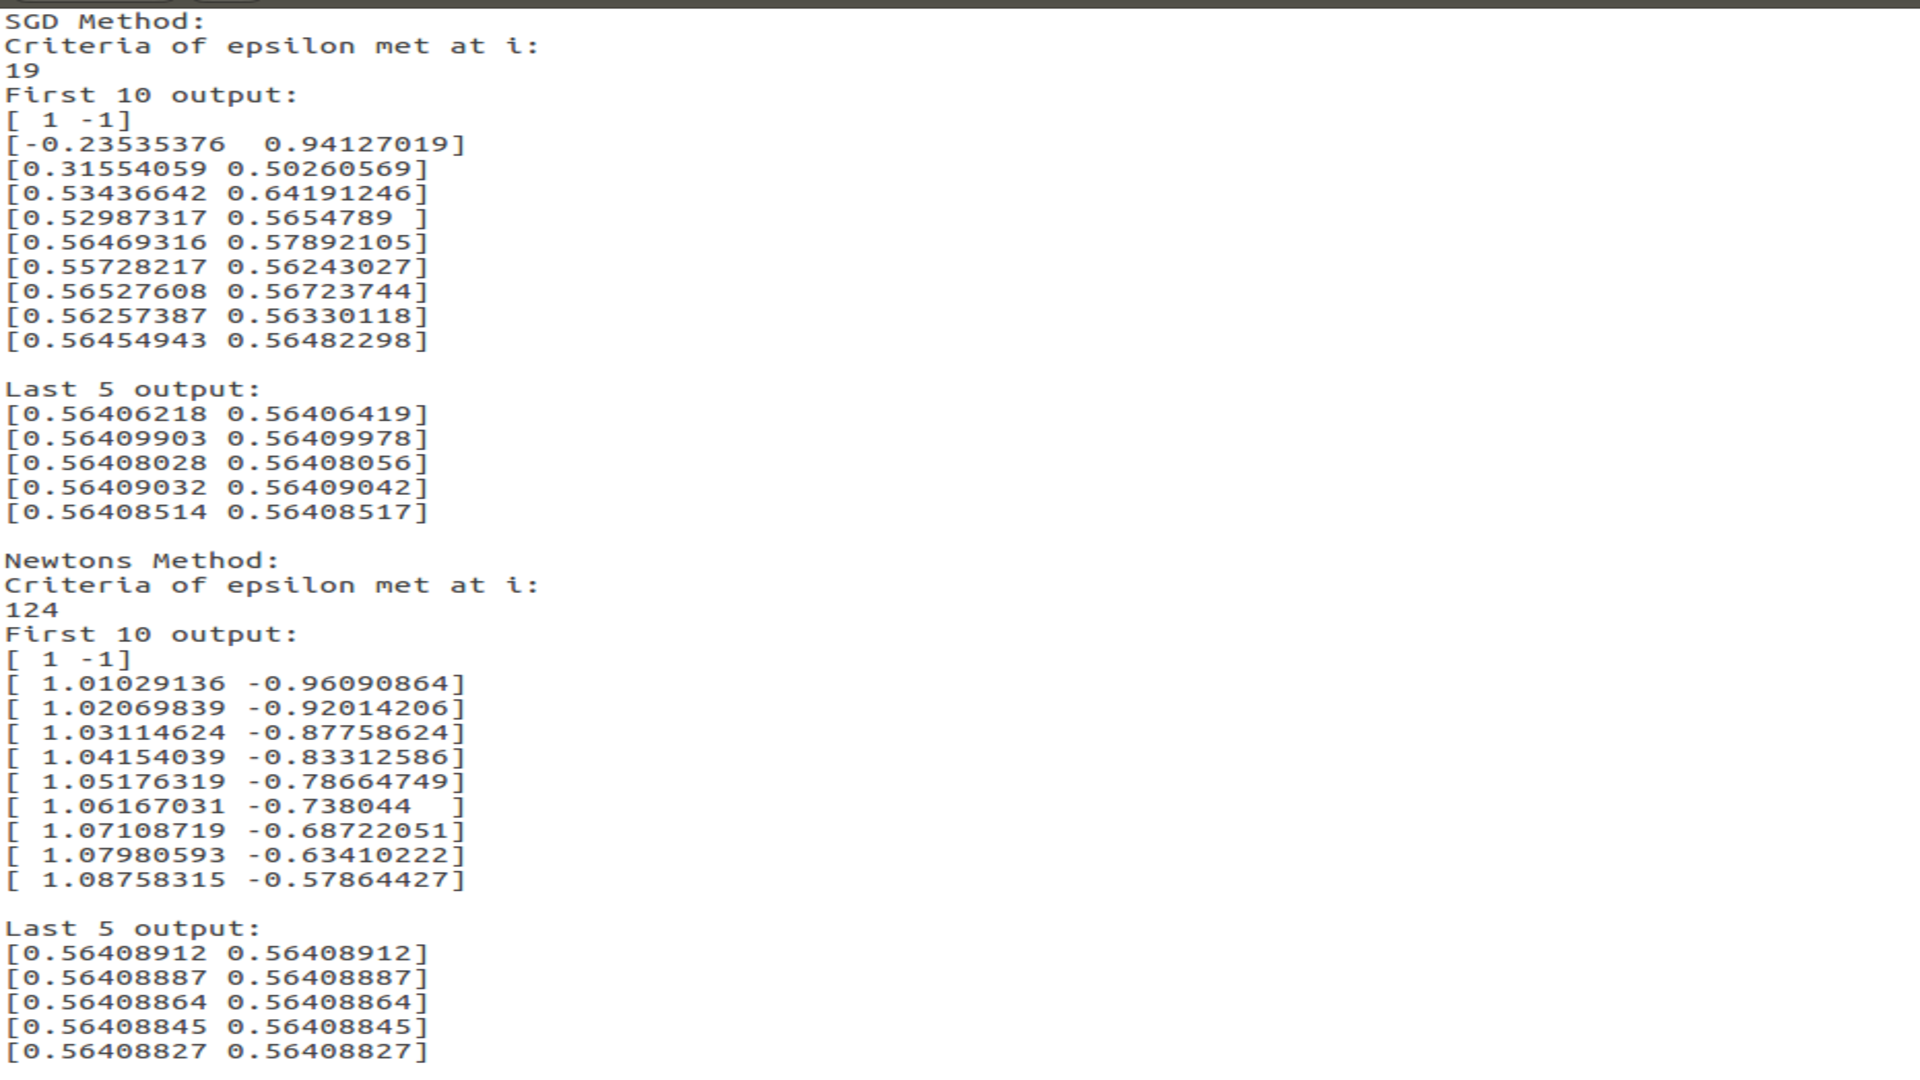
\includegraphics[width=0.25\textwidth]{out11.png}
\label{out11}
\end{figure}
\begin{figure}[H]
\caption{Output of BFGS and CGD optimization for C=1}
\centering
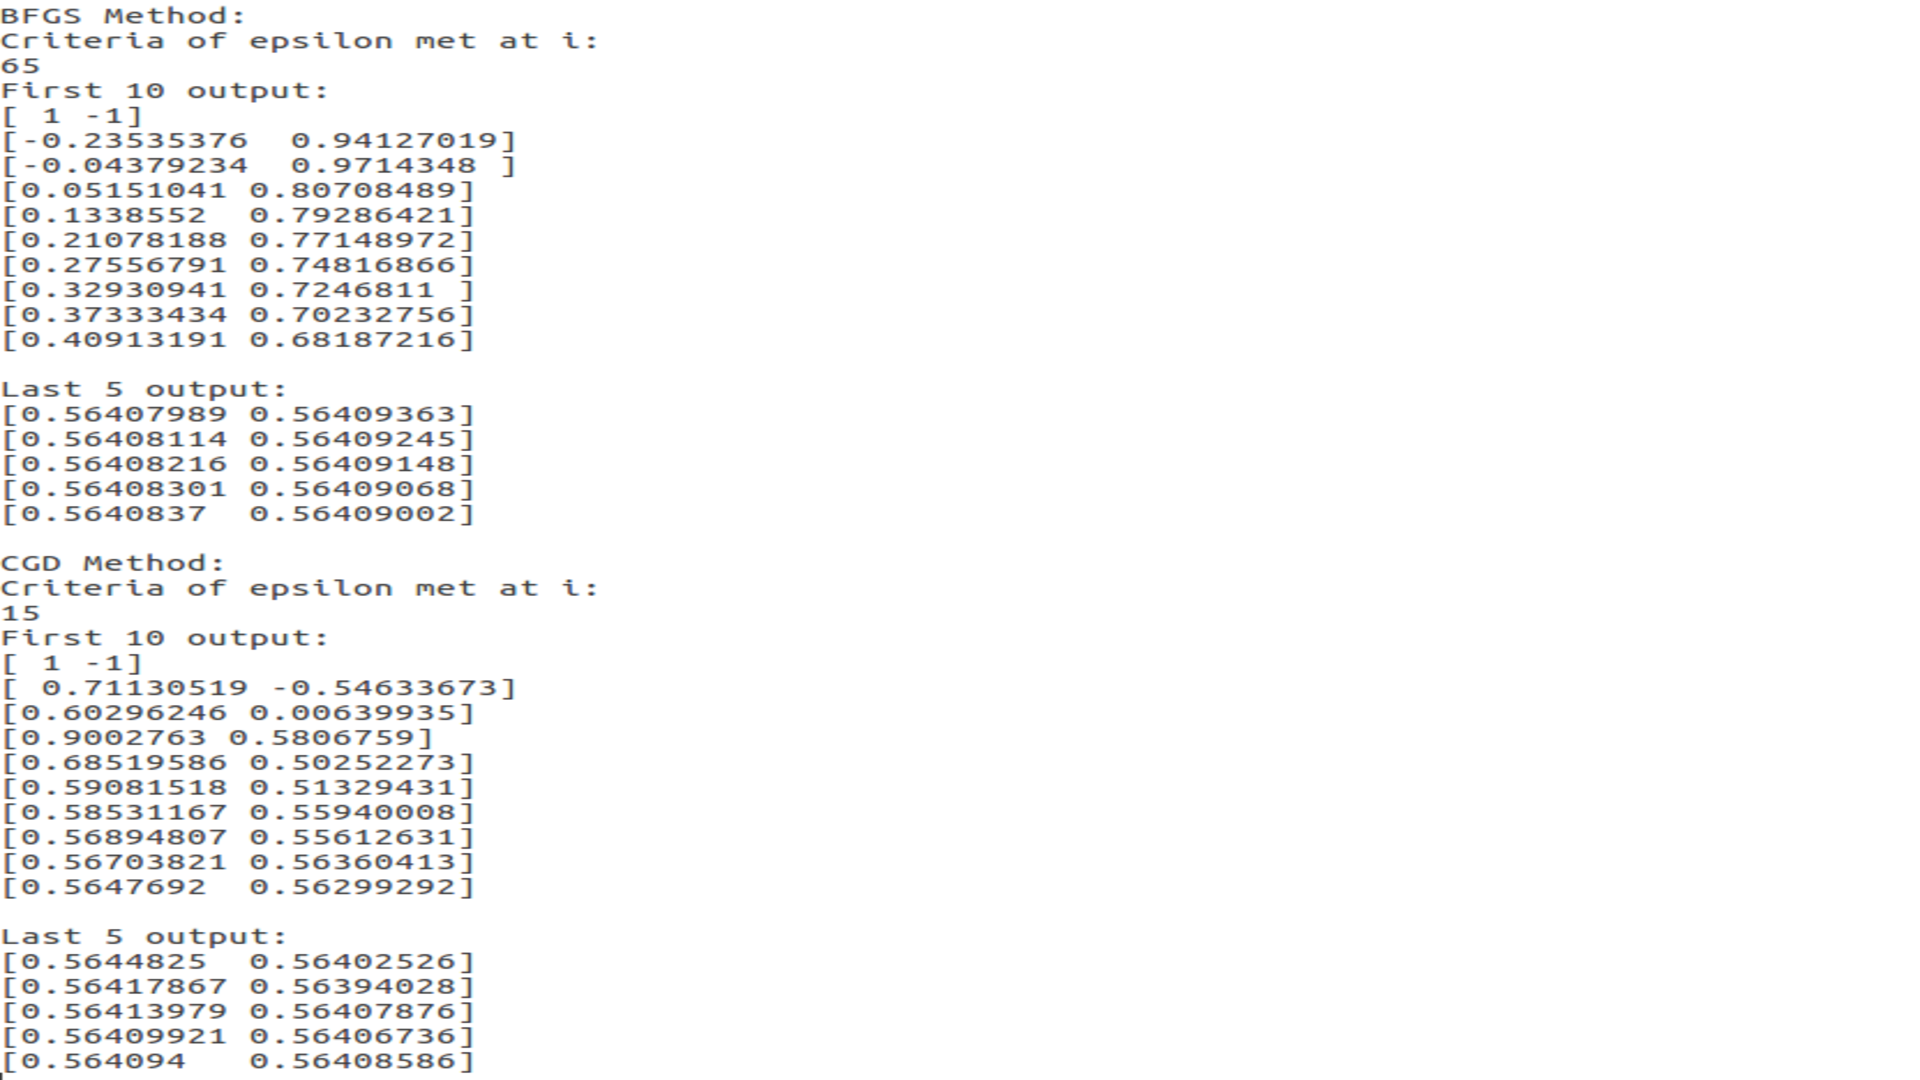
\includegraphics[width=0.25\textwidth]{out12.png}
\label{out12}
\end{figure}
\begin{figure}[H]
\caption{Output of SGD and Newton optimization for C=10}
\centering
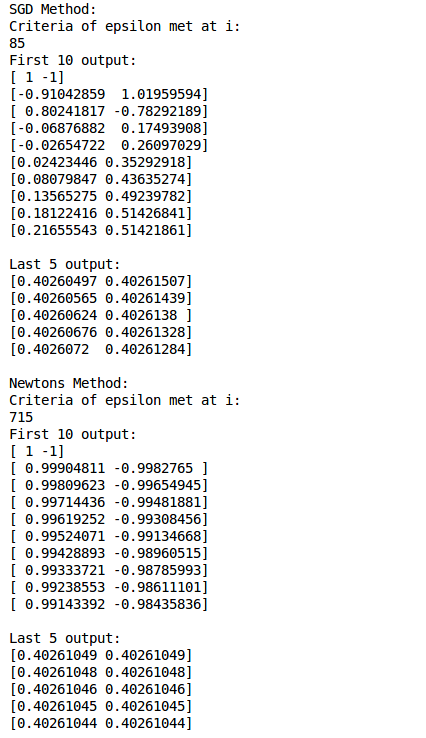
\includegraphics[width=0.25\textwidth]{out13.png}
\label{out13}
\end{figure}
\begin{figure}[H]
\caption{Output of BFGS and CGD optimization for C=10}
\centering
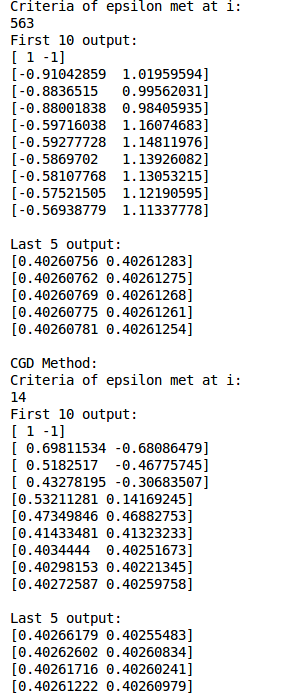
\includegraphics[width=0.25\textwidth]{out14.png}
\label{out14}
\end{figure}
\begin{figure}[H]
\caption{Output of SGD and Newton optimization for C=100}
\centering
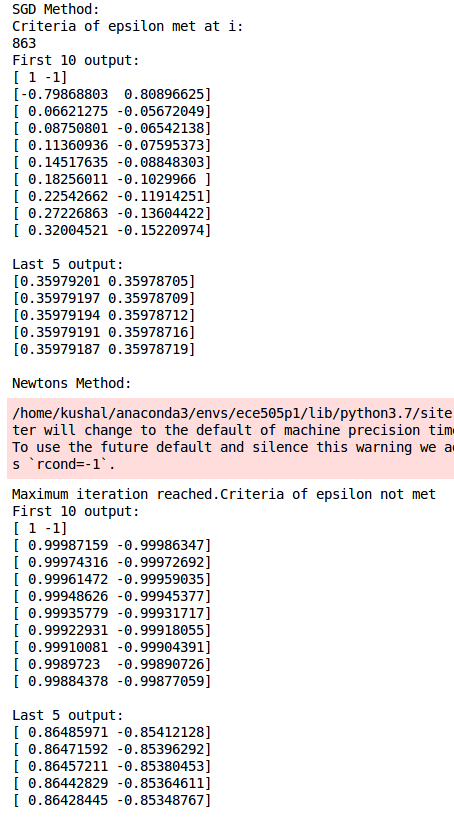
\includegraphics[width=0.25\textwidth]{out15.png}
\label{out15}
\end{figure}
\begin{figure}[H]
\caption{Output of BFGS and CGD optimization for C=100}
\centering
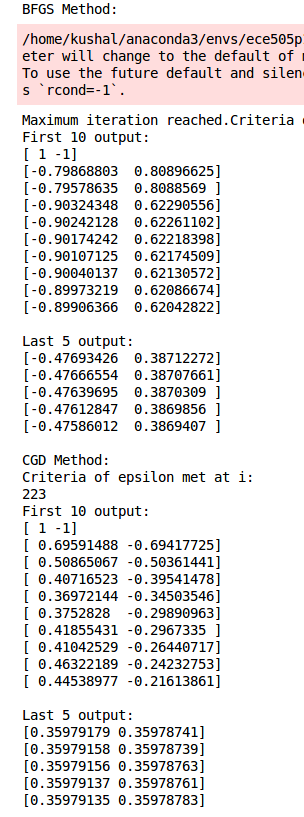
\includegraphics[width=0.25\textwidth]{out16.png}
\label{out16}
\end{figure}
\subsection*{Images of outputs for Optimization problem in Application Problem and Source Code}
\textbf{\url{https://github.com/kushalviit/Unconstrained_Optimization_ECE505/blob/master/project_notebook.ipynb}
Go to 7.Application (Optional) by scrolling down}
\begin{figure}[H]
\caption{Output of EM algorithm of Application Problem based on SGD method}
\centering
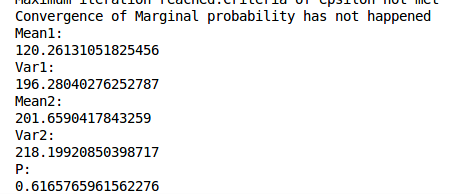
\includegraphics[width=0.25\textwidth]{out18.png}
\label{out18}
\end{figure}
\end{document}